\documentclass[letterpaper]{article}
\usepackage[polish]{babel} % Dodanie polskiego języka
\usepackage{geometry}
\usepackage{xcolor}
\usepackage{amsmath}
\usepackage[some]{background}
\usepackage{lipsum}
\usepackage[T1]{fontenc}
\usepackage[utf8]{inputenc}
\usepackage{tikz}
\usetikzlibrary{shapes.geometric, arrows.meta, positioning, fit}



\geometry{
    bottom=2cm % Ustawienie marginesu dolnego na 1 cm
}
\usepackage[geometry]{ifsym}

\definecolor{titlepagecolor}{cmyk}{1,.60,0,.40}

\backgroundsetup{
scale=1,
angle=0,
opacity=1,
contents={\begin{tikzpicture}[remember picture,overlay]
 \path [fill=titlepagecolor] (current page.west)rectangle (current page.north east); 
 \draw [color=white, very thick] (5,0)--(5,0.5\paperheight);
\end{tikzpicture}}
}

\makeatletter                   
\def\printauthor{%                  
    {\large \@author}}          
\makeatother

\author{%
    Jakub Iwaszkiewicz 264506 \\
    \texttt{264506@student.pwr.edu.pl}\vspace{40pt} \\
    Krzysztof Marszałek 263835 \\
    \texttt{263835@student.pwr.edu.pl}
    }

\begin{document}
\begin{titlepage}
    \BgThispage
    \newgeometry{left=1cm,right=6cm,bottom=2cm}
    \vspace*{0.4\textheight}
    \noindent

    \textcolor{white}{\Huge\textbf{\textsf{Dostęp do drzwi}}}
    \vspace*{2cm}\par
    \noindent
    \begin{minipage}{0.35\linewidth}
        \begin{flushright}
            \printauthor
        \end{flushright}
    \end{minipage} \hspace{15pt}
    %
    \begin{minipage}{0.02\linewidth}
        \rule{1pt}{175pt}
    \end{minipage} \hspace{-10pt}
    %
    \begin{minipage}{0.63\linewidth}
    \vspace{5pt}
        \begin{abstract} 
            System ma na celu udostępnienie panelu pozwalającego na nadawanie dostępu do pomieszczeń w zakładzie pracy (np. przez kontrolę kart zbliżeniowych). Z systemu mogą korzystać wyłącznie zalogowani użytkownicy. Pracownik uzyskuje informację o pomieszczeniach, do których ma uprawnienia, oraz może zgłosić zgubienie karty. Administrator systemu nadaje uprawnienia dostępowe dla użytkowników. Opcjonalnie, system powinien gromadzić informację o wykorzystaniu karty.       
        \end{abstract}
    \end{minipage}
    \end{titlepage}

\restoregeometry

\tableofcontents
\newpage
\section{Opis projektu}
\subsection{Skład grupy}
\begin{enumerate}
    \item Jakub Iwaszkiewicz - React.js, Node.js, MySQL, Express.js
    \item Krzysztof Marszałek - React.js, styles, MySQL
\end{enumerate}

\subsection{Cel projektu}
\noindent Celem projektu jest stworzenie nowoczesnej 
aplikacji internetowej, która poprawi efektywność i wydajność 
zarządzania dostępem do drzwi. Aplikacja "dostęp do drzwi" jest dla zakładu 
pracy i umożliwia dostęp do drzwi dla pracowników, który obecnie są w nim zatrudnieni. 
Aplikacja jest przeznaczona dla intranetu danego zakładu pracy. Użytkownicy niezalogowani 
mogą zalogować się jako pracownicy lub jak administrator, w zależności od tego czy dany 
użytkownik odpowiada za dostęp do drzwi. Administrator ma dostęp do wszystkich informacji 
jak i usług w firmie, czyli: może przyznawać dostępy do drzwi dla pracowników, może także 
usuwać te dostępy. Dodatkowo w każdej chwili może zmienić uprawienenia dostępu do drzwi w 
zależności od różnych sytuacji. Administrator dostaje prośbe o dostęp do drzwi w formie 
powiadomienia w momencie kiedy pracownik ją wyśle. Może zaakceptować albo anulować request. 
Co również odróznia administratora to fakt, że ma on wgląd w całą historie przyznawania 
dostępu do drzwi, przez siebie jak i przez innych administratorów. Pracownik może odcztać
 jakie ma przyznane dostępy do drzwi oraz wysłać prośbe o dostęp do nowych i tę prośbe 
 również usunąć. Projekt ma na celu nie tylko stworzenie funkcjonalnej 
 aplikacji, ale także zdobycie doświadczenia w pracy zespołowej i rozwijanie 
 umiejętności w zakresie nowoczesnych technologii webowych.

 \subsection{Typy użytkowników}
    \begin{enumerate}
        \item \textbf{Właściciel} \\
Właściciel jest użytkownikiem, który ma dostęp do wszystkich funkcjonalności systemu. Może on zarządzać użytkownikami, drzwiami, dostępami do drzwi oraz administratorami.


        \item \textbf{Administrator}\\
Administrator jest użytkownikiem, który ma dostęp do wszystkich funkcjonalności systemu. Może on zarządzać użytkownikami, drzwiami oraz dostępami do drzwi.       

        \item \textbf{Pracownik} \\
Pracownik jest użytkownikiem, który ma dostęp do uprawnień przyznanych przez administratora. 
        \item \textbf{Niezalogowany użytkownik} \\
Niezalogowany użytkownik nie ma dostępu do żadnych funkcjonalności systemu. Może on jedynie zalogować się do systemu.
    \end{enumerate}
\newpage
\section{Wymagania funkcjonalne}
\subsection{Logowanie}
\begin{enumerate}
    \item \textbf{Opis:} Użytkownik może zalogować się do systemu.
    \item \textbf{Aktorzy:} Niezalogowany użytkownik.
    \item \textbf{Scenariusz główny:} 
    \begin{enumerate}
        \item Użytkownik wypełnia formularz logowania.
        \item Użytkownik klika przycisk "Zaloguj".
        \item System sprawdza poprawność danych.
        \item System loguje użytkownika.
    \end{enumerate}
    \item \textbf{Scenariusz alternatywny:} 
    \begin{enumerate}
        \item Użytkownik wypełnia formularz logowania.
        \item Użytkownik klika przycisk "Zaloguj".
        \item System sprawdza poprawność danych.
        \item System wyświetla komunikat o błędzie.
    \end{enumerate}
\end{enumerate}
\subsection{Wylogowanie}
\begin{enumerate}
    \item \textbf{Opis:} Użytkownik może wylogować się z systemu.
    \item \textbf{Aktorzy:} Zalogowany użytkownik.
    \item \textbf{Scenariusz główny:} 
    \begin{enumerate}
        \item Użytkownik klika przycisk "Wyloguj" w panelu sterowania.
        \item System wylogowuje użytkownika i przekierowuje na stronę logowania.
    \end{enumerate}
\end{enumerate}

\subsection{Tworzenie drzwi}
\begin{enumerate}
    \item \textbf{Opis:} Administrator może dodać drzwi do systemu.
    \item \textbf{Aktorzy:} Administrator.
    \item \textbf{Scenariusz główny:} 
    \begin{enumerate}
        \item Administrator klika przycisk "Edytuj drzwi" w panelu sterowania.
        \item System wyświetla formularz dodawania drzwi.
        \item Administrator wypełnia formularz dodawania drzwi.
        \item Administrator klika przycisk "Dodaj".
        \item System sprawdza poprawność danych.
        \item System dodaje drzwi do systemu.
    \end{enumerate}
    \item \textbf{Scenariusz alternatywny:} 
    \begin{enumerate}
        \item Administrator klika przycisk "Edytuj drzwi" w panelu sterowania.
        \item System wyświetla formularz dodawania drzwi.
        \item Administrator wypełnia formularz dodawania drzwi.
        \item Administrator klika przycisk "Dodaj".
        \item System sprawdza poprawność danych.
        \item System wyświetla komunikat o błędzie.
    \end{enumerate}
\end{enumerate}

\subsection{Usuwanie drzwi}
\begin{enumerate}
    \item \textbf{Opis:} Administrator może usunąć drzwi z systemu.
    \item \textbf{Aktorzy:} Administrator.
    \item \textbf{Scenariusz główny:} 
    \begin{enumerate}
        \item Administrator klika przycisk "Edytuj drzwi" w panelu sterowania.
        \item System wyświetla formularz usuwania drzwi.
        \item Administrator wypełnia formularz usuwania drzwi.
        \item Administrator klika przycisk "Usuń".
        \item System sprawdza poprawność danych.
        \item System usuwa drzwi z systemu.
    \end{enumerate}
    \item \textbf{Scenariusz alternatywny:} 
    \begin{enumerate}
        \item Administrator klika przycisk "Edytuj drzwi" w panelu sterowania.
        \item System wyświetla listę isniejących drzwi
        \item Administrator klika przycisk "Usuń".
        \item System sprawdza poprawność danych.
        \item System wyświetla komunikat o błędzie.
    \end{enumerate}
\end{enumerate}

\subsection{Tworzenie konta pracowników}
\begin{enumerate}
    \item \textbf{Opis:} Administrator może dodać konto pracownika do systemu.
    \item \textbf{Aktorzy:} Administrator.
    \item \textbf{Scenariusz główny:} 
    \begin{enumerate}
        \item Administrator klika przycisk "Edytuj pracowników" w panelu sterowania.
        \item System wyświetla formularz dodawania pracownika.
        \item Administrator wypełnia formularz dodawania pracownika.
        \item Administrator klika przycisk "Dodaj".
        \item System sprawdza poprawność danych.
        \item System dodaje konto pracownika do systemu.
    \end{enumerate}
    \item \textbf{Scenariusz alternatywny:} 
    \begin{enumerate}
        \item Administrator klika przycisk "Edytuj pracowników" w panelu sterowania.
        \item System wyświetla formularz dodawania pracownika.
        \item Administrator wypełnia formularz dodawania pracownika.
        \item Administrator klika przycisk "Dodaj".
        \item System sprawdza poprawność danych.
        \item System wyświetla komunikat o błędzie.
    \end{enumerate}
\end{enumerate}

\subsection{Usuwanie konta pracownika}
\begin{enumerate}
    \item \textbf{Opis:} Administrator może usunąć konto pracownika z systemu.
    \item \textbf{Aktorzy:} Administrator.
    \item \textbf{Scenariusz główny:} 
    \begin{enumerate}
        \item Administrator klika przycisk "Edytuj pracowników" w panelu sterowania.
        \item System wyświetla liste isniejących pracowników.
        \item Administrator klika przycisk "Usuń".
        \item System sprawdza poprawność danych.
        \item System usuwa konto pracownika z systemu.
    \end{enumerate}
\end{enumerate}

\subsection{Przyznawanie uprawnień pracownikom do drzwi}
\begin{enumerate}
    \item \textbf{Opis:} Administrator może przyznać uprawnienia pracownikowi do drzwi.
    \item \textbf{Aktorzy:} Administrator.
    \item \textbf{Scenariusz główny:} 
    \begin{enumerate}
        \item Administrator klika przycisk "Edytuj dostępy" w panelu sterowania.
        \item System wyświetla dwie listy rozwijane: lista pracowników i lista drzwi.
        \item Administrator wybiera pracownika i drzwi, które chce mu przydzielić.
        \item Administrator klika przycisk "Przydziel dostęp".
        \item System sprawdza poprawność danych.
        \item System zapisuje zmiany.
    \end{enumerate}
    \item \textbf{Scenariusz alternatywny:}
    \item \begin{enumerate}
        \item Administrator klika przycisk "Edytuj dostępy" w panelu sterowania.
        \item System wyświetla dwie listy rozwijane: lista pracowników i lista drzwi.
        \item Administrator wybiera pracownika i drzwi, które chce mu przydzielić.
        \item Administrator klika przycisk "Przydziel dostęp".
        \item System sprawdza poprawność danych.
        \item System wyświetla komunikat o błędzie.
    \end{enumerate}
\end{enumerate}

\subsection{Usuwanie uprawnień pracownikom do drzwi}
\begin{enumerate}
    \item \textbf{Opis:} Administrator może usunąć uprawnienia pracownikowi do drzwi.
    \item \textbf{Aktorzy:} Administrator.
    \item \textbf{Scenariusz główny:} 
    \begin{enumerate}
        \item Administrator klika przycisk "Edytuj dostępy" w panelu sterowania.
        \item System wyświetla listę isniejących uprawnień.
        \item Administrator wybiera pracownika i drzwi, których uprawnienia chce mu odebrać.
        \item Administrator klika przycisk "Usuń".
        \item System sprawdza poprawność danych.
        \item System zapisuje zmiany.
    \end{enumerate}
\end{enumerate}

\subsection{Wyświetlanie dostępów pracownika}
\begin{enumerate}
    \item \textbf{Opis:} Pracownik może wyświetlić listę drzwi, do których ma dostęp pracownik.
    \item \textbf{Aktorzy:} Pracownik
    \item \textbf{Scenariusz główny:} 
    \begin{enumerate}
        \item Administrator klika przycisk ``Dostępy" w panelu sterowania.
        \item System wyświetla listę drzwi, do których ma dostęp pracownik.
    \end{enumerate}
\end{enumerate}

todo: dodac funkcjonalnosc gubienia karty
% dodamy ta funckoinalnosc w przyszlosci
% \subsection{Zgłoszenie zgubienia karty dostępu}
% \begin{enumerate}
%     \item \textbf{Opis:} Pracownik może zgłosić zgubienie karty dostępu.
%     \item \textbf{Aktorzy:} Pracownik
%     \item \textbf{Scenariusz główny:} 
%     \begin{enumerate}
%         \item Pracownik klika przycisk "Zgłoś zgubienie karty" w panelu sterowania.
%         \item System wyświetla formularz zgłoszenia zgubienia karty.
%         \item Pracownik wypełnia formularz zgłoszenia zgubienia karty.
%         \item Pracownik klika przycisk "Zgłoś".
%         \item System sprawdza poprawność danych.
%         \item System zapisuje zgłoszenie.
%     \end{enumerate}
%     \item \textbf{Scenariusz alternatywny:} 
%     \begin{enumerate}
%         \item Pracownik klika przycisk "Zgłoś zgubienie karty" w panelu sterowania.
%         \item System wyświetla formularz zgłoszenia zgubienia karty.
%         \item Pracownik wypełnia formularz zgłoszenia zgubienia karty.
%         \item Pracownik klika przycisk "Zgłoś".
%         \item System sprawdza poprawność danych.
%         \item System wyświetla komunikat o błędzie.
%     \end{enumerate}
% \end{enumerate}

\subsection{Zmiana właściciela systemu}
\begin{enumerate}
    \item \textbf{Opis:} Właściciel zmienia właściciela systemu.
    \item \textbf{Aktorzy:} Właściciel
    \item \textbf{Scenariusz główny:} 
    \begin{enumerate}
        \item Właściciel klika przycisk ``Dodaj przywieleje" w panelu sterowania.
        \item System wyświetla liste administartorów
        \item Administrator klika przycisk ``Ustaw jako ownera".
        \item System odbiera uprawnienia właściciela od aktualnego właściciela.
        \item System nadaje uprawnienia właściciela wybranemu administratorowi.
        \item System przeładuje stronę i były właściciel jest teraz zwykłym administratorem i nie możliwości zmiany właściciela.
    \end{enumerate}
\end{enumerate}
\section{Wykorzystane technologie}

\noindent Wykorzystana technologia: System kontroli wersji - Git

System kontroli wersji, który został wybrany do projektu to git. 
W znaczym stopniu ułatwił on pracę nad projektem. 
Pozwolił na łatwe śledzenie zmian w kodzie, 
a także na łatwe przywracanie poprzednich wersji. 
Dzięki niemu możliwa była również praca nad projektem 
przez dwie osoby jednocześnie. 

Stworzyliśmy repozytorium na platformie github.com.

\subsection{Wykorzystane technologie programistyczne}

\begin{itemize}
    \item \textbf{React.js}: Biblioteka React.js, która została wykorzystana do stworzenia i ustrukturyzowania interfejsu użytkownika przy pomocy JSX'a.
    \item \textbf{Express.js}: Biblioteka express.js, która została wykorzystana do stworzenia serwera, API i endpointów.
    \item \textbf{SASS}: Biblioteka SASS, która została wykorzystana do stylizacji interfejsu użytkownika.
    \item \textbf{Prisma}: ORM, który został wykorzystany do połączenia się, wykonywania zmian jak i komunikacji z bazą danych.
    \item \textbf{AWS}: Chmura AWS, która została wykorzystana do hostowania bazy danych.
    \item \textbf{REST}: Architektura REST, która została wykorzystana do komunikacji między serwerem a klientem. 
    \item \textbf{Figma}: Program Figma, który został wykorzystany do stworzenia projektu interfejsu użytkownika.
    \item \textbf{Visual Studio Code}: Środowisko programistyczne Visual Studio Code, które zostało wykorzystane do pisania kodu serwera, kodu aplikacji jak i kodu dokumentacji.
    \item \textbf{LaTeX}: Środowisko programistyczne LaTeX, które zostało wykorzystane do pisania dokumentacji.
\end{itemize}

\section{Architektura informacji}
\subsection{Schemat bazy danych}
\begin{figure}[h]
    \centering
    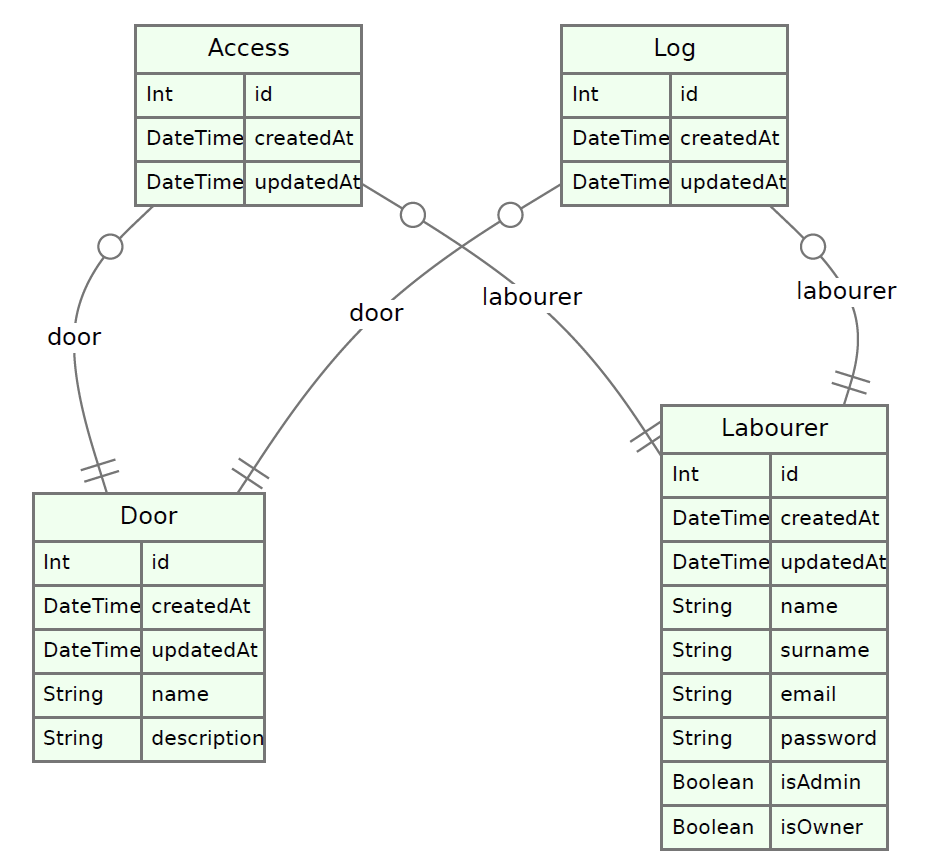
\includegraphics[scale=0.6]{photos/schemat_bazy_danych.png}
    \caption{Schemat bazy danych}
    \label{fig:erd}
\end{figure}
\newpage
\subsection{Stworzenie bazy danych}



\subsection{Opis encji w bazie dancyh}

\subsubsection{Tabela Labourers}
\noindent Tabela zawierająca wszystkie informacje dotyczących użytjowników aplikacji - są w 
w niej zawarte informacje o użytkownikach, którzy są pracownikami, 
administratorami i właścicielami.
\begin{table}[h]
    \centering
    \scalebox{0.75}{
    \begin{tabular}{|c|c|c|c|c|c|c|c|c|}
    \hline
    \textbf{id} & \textbf{createdAt} & \textbf{updatedAt} & \textbf{name} & \textbf{surname} & \textbf{email} & \textbf{passowrd} & \textbf{isAdmin} & \textbf{isOwner} \\ \hline
    int AI PK   & datetime(3)        & datetime(3)        & varchar(191)  & varchar(191)     & varchar(191)   & varchar(191)      & tinyint(1)       & tinyint(1)       \\ \hline
    \end{tabular}}
    \caption{Tabela Labourers}
    \end{table}


\subsubsection{Tabela Door}
\noindent Tabela zawierająca wszystkie informacje dotyczące drzwi -
 są w niej zawarte informacje: kiedy zostały stworzone, kiedy zostały ostatnio do kogoś przypisane, 
 nazwa oraz opis drzwi.
 \begin{table}[h]
    \centering
    \scalebox{0.75}{
    \begin{tabular}{|c|c|c|c|c|}
    \hline
    \textbf{id} & \textbf{createdAt} & \textbf{updatedAt} & \textbf{name} & \textbf{description} \\ \hline
    int AI PK   & datetime(3)        & datetime(3)        & varchar(191)  & varchar(191)         \\ \hline
    \end{tabular}}
    \caption{Tabela Door}
\end{table}

\subsubsection{Tabela Access}
\noindent Tabela zawierająca wszystkie informacje dotyczące uprawnień do drzwi-
są zawarte w niej informacje: kiedy zostały stworzone, kiedy zostały ostatnio zmodyfikowane,
jakie drzwi są do jakiego użytkownika przypisane.
\begin{table}[h]
    \centering
    \scalebox{0.75}{
    \begin{tabular}{|c|c|c|c|c|}
    \hline
    \textbf{id} & \textbf{createdAt} & \textbf{updatedAt} & \textbf{doorID} & \textbf{labourerID} \\ \hline
    int AI PK   & datetime(3)        & datetime(3)        & int           & int               \\ \hline
    \end{tabular}}
    \caption{Tabela Access}
\end{table}

% \subsubsection{Tabela AccessAddedByLog}
% \noindent Tabela zawierająca wszystkie informacje dotyczące logów dodawania uprawnień do drzwi - SA
% są w niej zawarte informacje: kiedy zostały stworzone, kiedy zostały ostatnio zmodyfikowane, 
% indetyfikator dostępu, identyfikator administratora, identyfikator drzwi, do których zostały dodane uprawnienia.
% \begin{table}[h]
%     \centering
%     \scalebox{0.8}{
%     \begin{tabular}{|c|c|c|c|c|c|}
%     \hline
%     \textbf{id} & \textbf{createdAt} & \textbf{updatedAt} & \textbf{accessID} & \textbf{adminID} & \textbf{doorID} \\ \hline
%     int AI PK   & datetime(3)        & datetime(3)        & int             & int           & int              \\ \hline
%     \end{tabular}}
%     \caption{Tabela AccessAddedByLog}
% \end{table}


% \subsubsection{Tabela DoorOpenedLog}

% \noindent Tabela zawierająca wszystkie informacje dotyczące logów otwierania drzwi - 
% są w niej zawarte informacje: kiedy zostały stworzone, 
% kiedy zostały ostatnio zmodyfikowane, identyfikator drzwi
% oraz identyfikator użytkownika.  
% \begin{table}[h]
%     \centering
%     \scalebox{0.8}{
%     \begin{tabular}{|c|c|c|c|c|}
%     \hline
%     \textbf{id} & \textbf{createdAt} & \textbf{updatedAt} & \textbf{doorID} & \textbf{labourerID} \\ \hline
%     int AI PK   & datetime(3)        & datetime(3)        & int           & int               \\ \hline
%     \end{tabular}}
%     \caption{Tabela DoorOpenedLog}
% \end{table}


\section{Wprowadzenie do API}
\noindent API naszej aplikacji webowej są kluczowymi elementami
które umożliwiają interakcje pomiędzy front-endem a bazą danych. Dzięki nim
użytkownicy mogą wykonywać operacje na danych
takie jak: tworzenie, odczytywanie, aktualizowanie i usuwanie danych w responsywny sposób.


\subsection{Konfiguracja i użycie API}
\noindent Nasze API zostało zaprojektowane z myślą o łatwości integracji i elastyczności. W tej sekcji przedstawimy kluczowe aspekty konfiguracji i podstawowe kroki potrzebne 
do rozpoczęcia pracy z naszym API, w tym uwierzytelnianie i podstawowe zapytania.

\subsection{Endpointy API}
\begin{itemize}
    \item Tworzenie zasobów (Create Endpoints)
    \item Uusuwanie zasobów (Delete Endpoints)
    \item Odczyt zasobów (Read Endpoints)
    \item Aktualizacja zasobów (Update Endpoints)
\end{itemize}

\textbf{\large{Dodawanie Pracownika (Labourer)}}
\begin{itemize}
    \item \textbf{Metoda:} POST
    \item \textbf{Ścieżka:} '/labourers'
    \item \textbf{Autentykacja:} Wymagany token uwierzytelniający
    \item \textbf{Opis:} Pozwala na dodanie tylko administartorowi nowego pracownika do systemu. Wymaga podania danych takich jak:
        \begin{itemize}
        \item \textbf{name} - imię pracownika
        \item \textbf{surname} - nazwisko pracownika
        \item \textbf{email} - adres email pracownika
        \item \textbf{password} - hasło pracownika
        \end{itemize}
    \item \textbf{Walidacja:} Sprawdza, czy email i hasło spełniają określone kryteria (np. długość hasła, format emaila)
    \item \textbf{Odpowiedź:} Status 200 - OK przy udanym dodaniu, 403 Forbidden przy błędach walidacji lub braku uprawnień
\end{itemize}

\textbf{\large{Dodawanie Drzwi (Door)}}
\begin{itemize}
    \item \textbf{Metoda:} POST
    \item \textbf{Ścieżka:} '/doors'
    \item \textbf{Autentykacja:} Wymagany token uwierzytelniający
    \item \textbf{Opis:} Pozwala na dodanie tylko administartorowi nowych drzwi do systemu. Wymaga podania danych takich jak:
        \begin{itemize}
        \item \textbf{name} - nazwa drzwi
        \item \textbf{description} - opis drzwi
        \end{itemize}
    \item \textbf{Walidacja:} Sprawdza, czy nazwa drzwi jest unikalna
    \item \textbf{Odpowiedź:} Status 200 - OK przy udanym dodaniu, 403 Forbidden przy błędach walidacji lub braku uprawnień
\end{itemize}

\textbf{\large{Dodawanie Uprawnień (Access)}}
\begin{itemize}
    \item \textbf{Metoda:} POST
    \item \textbf{Ścieżka:} '/accesses'
    \item \textbf{Autentykacja:} Wymagany token uwierzytelniający
    \item \textbf{Opis:} Pozwala na dodanie tylko administartorowi nowych uprawnień do systemu. Sprawdza, czy dany pracownik i drzwi istnieją w systemie.
    \item \textbf{Odpowiedź:} Status 200 - OK przy udanym dodaniu, 403 Forbidden przy błędach walidacji lub braku uprawnień
\end{itemize}

\subsubsection{\textbf{\large{Usuwanie zasobów (Delete Endpoints)}}}
\textbf{\large{Usuwanie Pracownika (Labourer)}}
\begin{itemize}
    \item \textbf{Metoda:} DELETE
    \item \textbf{Ścieżka:} '/labourers'
    \item \textbf{Autentykacja:} Wymagany token uwierzytelniający
    \item \textbf{Opis:} Pozwala na usunięcie tylko administartorowi pracownika z systemu. Wymaga podania email pracownika.
    \item \textbf{Odpowiedź:} Status 200 - OK przy udanym usunięciu, 403 Forbidden przy błędach walidacji lub braku uprawnień.
\end{itemize}

\textbf{\large{Usuwanie Drzwi (Door)}}
\begin{itemize}
    \item \textbf{Metoda:} DELETE
    \item \textbf{Ścieżka:} '/doors'
    \item \textbf{Autentykacja:} Wymagany token uwierzytelniający
    \item \textbf{Opis:} Pozwala na usunięcie tylko administartorowi drzwi z systemu. Wymaga podania nazwy drzwi.
    \item \textbf{Odpowiedź:} Status 200 - OK przy udanym usunięciu, 403 Forbidden przy błędach walidacji lub braku uprawnień.
\end{itemize}

\textbf{\large{Usuwanie Uprawnień (Access)}}
\begin{itemize}
    \item \textbf{Metoda:} DELETE
    \item \textbf{Ścieżka:} '/access'
    \item \textbf{Autentykacja:} Wymagany token uwierzytelniający
    \item \textbf{Opis:} Pozwala na usunięcie tylko administartorowi uprawnień z systemu. Wymaga podania id pracownika i id drzwi.
    \item \textbf{Odpowiedź:} Status 200 - OK przy udanym usunięciu, 403 Forbidden przy błędach walidacji lub braku uprawnień.
\end{itemize}

\subsubsection{\textbf{\large{Odczyt zasobów (Read Endpoints)}}}
\textbf{\large{Odczyt wszystkich Pracowników (Labourers)}}
\begin{itemize}
    \item \textbf{Metoda:} GET
    \item \textbf{Ścieżka:} '/labourers'
    \item \textbf{Autentykacja:} Wymagany token uwierzytelniający
    \item \textbf{Opis:} Pozwala na odczyt tylko administartorowi pracowników z systemu.
    \item \textbf{Odpowiedź:} Zwraca listę pracowników w formacie JSON.
\end{itemize}

\textbf{\large{Odczyt danych o Pracowniku (Labourer)}}
\begin{itemize}
    \item \textbf{Metoda:} GET
    \item \textbf{Ścieżka:} '/labourer'
    \item \textbf{Autentykacja:} Wymagany token uwierzytelniający
    \item \textbf{Opis:} Umozliwa pracownikowi odczytanie własnych danych z systemu.
    \item \textbf{Odpowiedź:} Zwraca dane zalogowanego pracownika w formacie JSON.
\end{itemize}

\textbf{\large{Odczyt wszystkich Drzwi (Door)}}
\begin{itemize}
    \item \textbf{Metoda:} GET
    \item \textbf{Ścieżka:} '/doors'
    \item \textbf{Autentykacja:} Wymagany token uwierzytelniający
    \item \textbf{Opis:} Pozwala na odczyt tylko administartorowi wszystkich drzwi z systemu.
    \item \textbf{Odpowiedź:} Zwraca listę drzwi w formacie JSON.
\end{itemize}

\textbf{\large{Odczyt dostępów (Access)}}
\begin{itemize}
    \item \textbf{Metoda:} GET
    \item \textbf{Ścieżka:} '/access'
    \item \textbf{Autentykacja:} Wymagany token uwierzytelniający
    \item \textbf{Opis:} Pozwala na odczytanie pracownikowi odczytanie informacji o swoich uprawnieniach do drzwi. Z
    \item \textbf{Odpowiedź:} Zwraca listę uprawnień w formacie JSON, kazdy z dostępów zawiera nazwę drzwi.
\end{itemize}

\textbf{\large{Odczyt administratorów (Administrators)}}
\begin{itemize}
    \item \textbf{Metoda:} GET
    \item \textbf{Ścieżka:} '/administrators'
    \item \textbf{Autentykacja:} Wymagany token uwierzytelniający
    \item \textbf{Opis:} Pozwala na odczyt tylko właścicielowi wszystkich administratorów z systemu.
    \item \textbf{Odpowiedź:} Zwraca listę administratorów w formacie JSON.
\end{itemize}


\subsubsection{Aktualizacja zasobów (Update Endpoints)}
\textbf{\large{Dodanie uprawnień Administratora}}
\begin{itemize}
    \item \textbf{Metoda:} PUT
    \item \textbf{Ścieżka:} '/privileges/add'
    \item \textbf{Autentykacja:} Wymagany token uwierzytelniający z uprawieniami właścicielami.
    \item \textbf{Opis:} Pozwala właścicielowi aplikacji na przyznanie uprawnień administratora istniejącemu pracownikowi. Wymaga podania adresu email pracownika, który ma otrzymać uprawnienia.
    \item \textbf{Walidacja:}  Sprawdzane jest, czy zalogowany użytkownik jest właścicielem, czy podany email istnieje w systemie, i czy pracownik nie jest już administratorem.
    \item \textbf{Odpowiedź:}  Status 200 OK po udanym przyznaniu uprawnień, 403 Forbidden, jeśli użytkownik nie jest właścicielem, 404 Not Found, jeśli pracownik nie istnieje, 400 Bad Request, jeśli pracownik już jest administratorem.
\end{itemize}

\textbf{\large{Usunięcie uprawnień Administratora}}
\begin{itemize}
    \item \textbf{Metoda:} PUT
    \item \textbf{Ścieżka:} '/privileges/delete'
    \item \textbf{Autentykacja:} Wymagany token uwierzytelniający z uprawieniami właścicielami.
    \item \textbf{Opis:} Pozwala właścicielowi aplikacji na odebranie uprawnień administratora istniejącemu pracownikowi. Wymaga podania adresu email pracownika, który ma stracić uprawnienia.
    \item \textbf{Walidacja:}  Sprawdzane jest, czy zalogowany użytkownik jest właścicielem, czy podany email istnieje w systemie, i czy pracownik jest administratorem.
    \item \textbf{Odpowiedź:}  Status 200 OK po udanym odebraniu uprawnień, 403 Forbidden, jeśli użytkownik nie jest właścicielem, 404 Not Found, jeśli pracownik nie istnieje, 400 Bad Request, jeśli pracownik nie jest administratorem.
\end{itemize}

\textbf{\large{Transfer uprawnień Właściciela}}
\begin{itemize}
    \item \textbf{Metoda:} PUT
    \item \textbf{Ścieżka:} '/privileges/transfer'
    \item \textbf{Autentykacja:} Wymagany token uwierzytelniający z uprawieniami właścicielami.
    \item \textbf{Opis:} Umożliwia właścicielowi na przekazanie swoich uprawnień innemu administratorowi. Wymaga podania emaila pracownika, który ma otrzymać uprawnienia właściciela.
    \item \textbf{Walidacja:}  Sprawdzane jest, czy zalogowany użytkownik jest właścicielem, czy pracownik istnieje w systemie, i czy jest administratorem.
    \item \textbf{Odpowiedź:}  Status 200 OK po udanym transferze uprawnień, 403 Forbidden, jeśli użytkownik nie jest właścicielem, 404 Not Found, jeśli pracownik nie istnieje, 400 Bad Request, jeśli pracownik nie jest administratorem.
\end{itemize}


\subsubsection{Zestawienie graficzne endpointów}
\begin{center}
    \begin{tikzpicture}[
      endpoint/.style={
        rectangle, 
        rounded corners, 
        minimum width=3cm, 
        minimum height=1cm, 
        text centered, 
        draw=black, 
        fill=blue!30,
        text width=2.5cm
      },
      rolelabel/.style={
        fill=yellow!30,
        text centered,
        minimum width=3cm
      },
      arrow/.style={
        thick,
        ->,
        >=Stealth
      },
      node distance=0.8cm
    ]
    
    % Labourer Nodes
    \node (labourerRole) [rolelabel] {Labourer};
    \node (login) [endpoint, below=of labourerRole] {POST /login \\ Logowanie użytkownika};
    \node (readSelf) [endpoint, below=of login] {GET /labourer \\ Odczyt danych pracownika};
    \node (readAccess) [endpoint, below=of readSelf] {GET /access \\ Odczyt uprawnień pracownika};
    
    % Administrator Nodes
    \node (adminRole) [rolelabel, right=of labourerRole] {Administrator};
    \node (createLabourerAdmin) [endpoint, right=of login] {POST /labourer \\ Dodanie pracownika};
    \node (deleteLabourerAdmin) [endpoint, below=of createLabourerAdmin] {DELETE /labourer \\ Usunięcie pracownika};
    \node (createDoorAdmin) [endpoint, below=of deleteLabourerAdmin] {POST /door \\ Dodanie drzwi};
    \node (deleteDoorAdmin) [endpoint, below=of createDoorAdmin] {DELETE /door \\ Usunięcie drzwi};
    \node (createAccessAdmin) [endpoint, below=of deleteDoorAdmin] {POST /access \\ Dodanie dostępu};
    \node (deleteAccessAdmin) [endpoint, below=of createAccessAdmin] {DELETE /access \\ Usunięcie dostępu};
    \node (readDoorsAdmin) [endpoint, below=of deleteAccessAdmin] {GET /doors \\ Odczyt wszystkich drzwi};
    \node (readAccessesAdmin) [endpoint, below=of readDoorsAdmin] {GET /accesses \\ Odczyt wszystkich dostępów};
    \node (readAllAdmin) [endpoint, below=of readAccessesAdmin] {GET /labourers \\ Odczyt wszystkich pracowników};
    
    % Owner Nodes
    \node (ownerRole) [rolelabel, right=of adminRole] {Owner};
    \node (deletePrivilegesOwner) [endpoint, right=of createLabourerAdmin] {PUT /privileges/delete \\ Usunięcie uprawnień admina};
    \node (transferPrivilegesOwner) [endpoint, below=of deletePrivilegesOwner] {PUT /privileges/transfer \\ Transfer uprawnień właściciela};
    \node (ownerEndpoints) [endpoint, below=of transferPrivilegesOwner, yshift=-2cm] {Wszystkie endpointy \\ Administratora i więcej};
    
    % Arrows for Labourer
    \draw [arrow] (labourerRole) -- (login);
    \draw [arrow] (login) -- (readSelf);
    \draw [arrow] (readSelf) -- (readAccess);
    
    % Arrows for Administrator
    \draw [arrow] (adminRole) -- (createLabourerAdmin);
    \draw [arrow] (createLabourerAdmin) -- (deleteLabourerAdmin);
    \draw [arrow] (deleteLabourerAdmin) -- (createDoorAdmin);
    \draw [arrow] (createDoorAdmin) -- (deleteDoorAdmin);
    \draw [arrow] (deleteDoorAdmin) -- (createAccessAdmin);
    \draw [arrow] (createAccessAdmin) -- (deleteAccessAdmin);
    \draw [arrow] (deleteAccessAdmin) -- (readDoorsAdmin);
    \draw [arrow] (readDoorsAdmin) -- (readAccessesAdmin);
    \draw [arrow] (readAccessesAdmin) -- (readAllAdmin);
    
    % Box around Labourer Nodes
    \node (labourerBox) [draw=red, dashed, fit=(labourerRole) (login) (readSelf) (readAccess), inner sep=0.3cm] {};
    
    % Box around Administrator Nodes
    \node (adminBox) [draw=red, dashed, fit=(adminRole) (createLabourerAdmin) (deleteLabourerAdmin) (createDoorAdmin) (deleteDoorAdmin) (createAccessAdmin) (deleteAccessAdmin) (readDoorsAdmin) (readAccessesAdmin) (readAllAdmin), inner sep=0.3cm] {};
    
    % Box around Owner Nodes
    \node (ownerBox) [draw=red, dashed, fit=(ownerRole) (deletePrivilegesOwner) (transferPrivilegesOwner) (ownerEndpoints), inner sep=0.3cm] {};
    
    \end{tikzpicture}
    \end{center}
    
\section{Konfiguracja serwera}
\begin{enumerate}
    \item Środowisko i konfiguracja:
        \begin{itemize}
            \item dotenv - Wykorzystanie pakietu dotenv do zarządzania 
            zmiennymi środowiskowymi, co ułatwia konfigurację aplikacji bez bezpośredniego umieszczania wrażliwych danych w kodzie.
            \item Port - Serwer jest skonfigurowany do nasłuchiwania na porcie określonym w zmiennej środowiskowej PORT, z domyślnym fallbackiem na port 3002.
        \end{itemize}
    \item Middleware
        \begin{itemize}
            \item CORS: Konfiguracja Cross-Origin Resource Sharing (CORS) ogranicza żądania do zaufanych domen (tutaj http://localhost:5173), zezwalając na metody HTTP takie jak GET, POST, DELETE itp. Jest to istotne z punktu widzenia 
            \item JSON Parser: Użycie express.json() jako middleware do parsowania przychodzących żądań z treścią w formacie JSON.
        \end{itemize}
    \item Routing
        \begin{itemize}
            \item Read Routes: Import i użycie route'ów do odczytu danych (readRoutes) pod ścieżką /api/read.
            \item Create Routes: Import i użycie route'ów do tworzenia danych (createRoutes) pod ścieżką /api/create.
            \item Delete Routes: Import i użycie route'ów do usuwania danych (deleteRoutes) pod ścieżką /api/delete.
            \item Update Routes: Import i użycie route'ów do aktualizacji danych (updateRoutes) pod ścieżką /api/update.
        \end{itemize}
    \item Generowanie Tokenów JWT
        \begin{itemize}
            \item Tokeny te są wykorzystywane do uwierzytelniania i zarządzania sesjami użytkowników.
        \end{itemize}
    \item Konfiguracja ORM Prisma
        \begin{itemize}
            \item Prisma jest ORM (Object Relational Mapping) do Node.js i TypeScript, który umożliwia bezpośredni dostęp do bazy danych z poziomu kodu źródłowego aplikacji.
            \item Prisma Client jest generowany na podstawie schematu bazy danych, który jest zdefiniowany w pliku schema.prisma.
            \item Użyto MySQL jako bazy danych.
            \item Prisma jest skonfigurowana do połączenia z bazą danych za pomocą zmiennej środowiskowej DATABASE\_URL.
        \end{itemize}
\end{enumerate}
\newpage
\section{Graficzny projekt interfejsu użytkownika}

\subsection{Ekran logowania}
\noindent Pierwszym widokiem, który widzi użytkownik po wejściu na stronę jest ekran logowania. 
Na środku konterena znajduje się nazwa aplikacji, a pod nią formularz logowania. 
W celu potwierdzenia logowania należy kliknąć przycisk "Zaloguj się".
\begin{figure}[h]
    \centering
    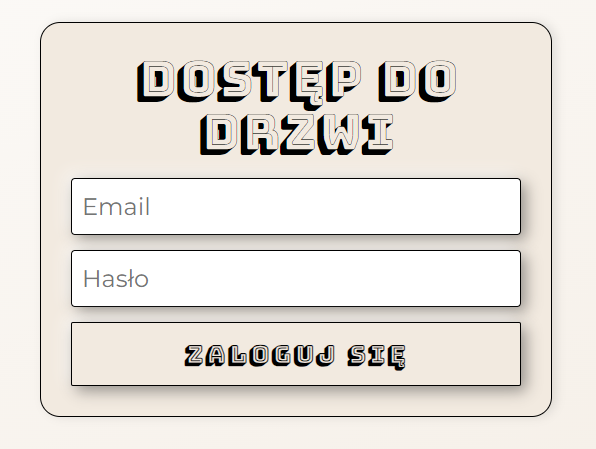
\includegraphics[scale=0.7]{photos/ekran_logowania.png}
    \caption{Ekran logowania}
    \label{fig:login}
\end{figure}

\noindent W przypadku niepoprawnego wprowadzenia danych, użytkownik zostanie poinformowany
 o błędnym formacie emaila:
\begin{figure}[h]
    \centering
    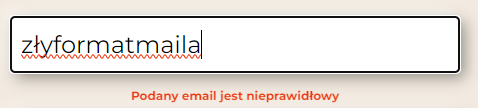
\includegraphics[scale=0.7]{photos/zlymail.png}
    \caption{Ekran logowania - błędny email}
    \label{fig:login}
\end{figure}

\noindent Analogicznie po wprowadzeniu błędnego hasła wyświetli się następujący komunikat:
\begin{figure}[h]
    \centering
    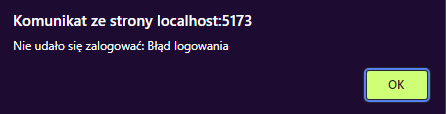
\includegraphics[scale=0.7]{photos/zle_haslo.png}
    \caption{Ekran logowania - błędne hasło}
    \label{fig:login}
\end{figure}
\newpage
\subsection{Profil pracownika}
Pracownik po zalogowaniu się do systemu zostanie przekierowany na strone swojego profilu,
gdzie zostają mu wyśwetlone informacje o nim:
\begin{figure}[h]
    \centering
    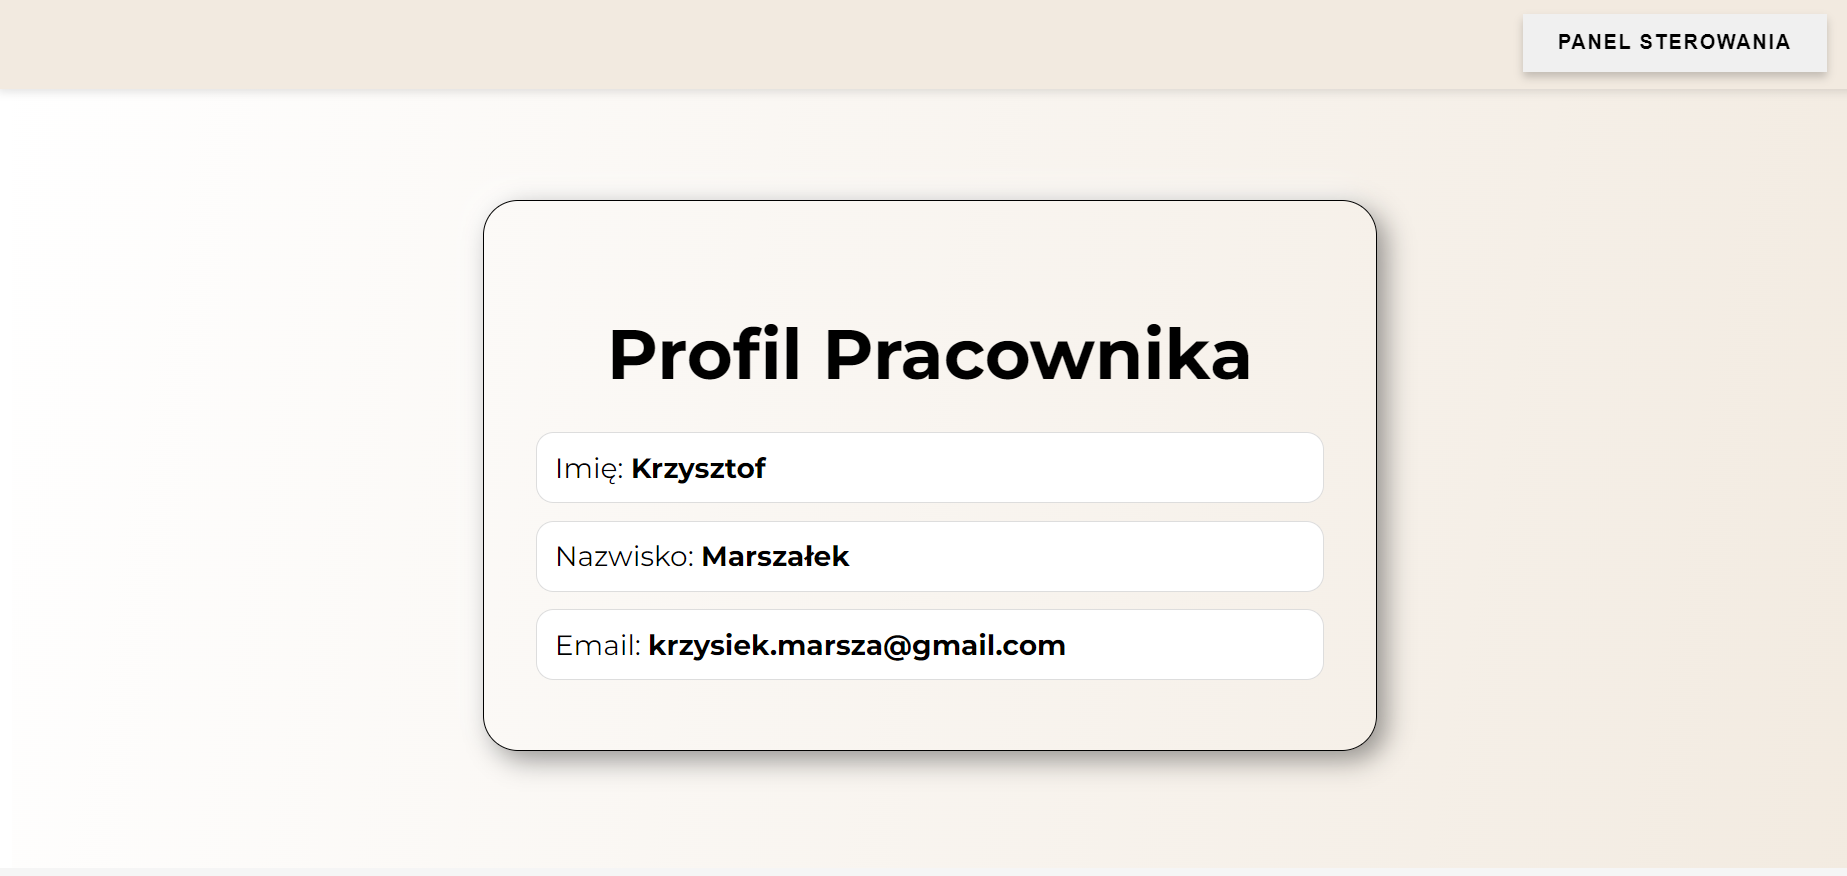
\includegraphics[scale=0.3]{photos/profil_pracownika.png}
    \caption{Profil pracownika}
    \label{fig:login}
\end{figure}


\noindent W prawym górnym rogu znajduje się tzw. hamburger menu pod nazwa "Panel sterowania", które po kliknięciu
rozwinie się i pokaże opcje, które są dostępne dla pracownika:
\begin{figure}[h]
    \centering
    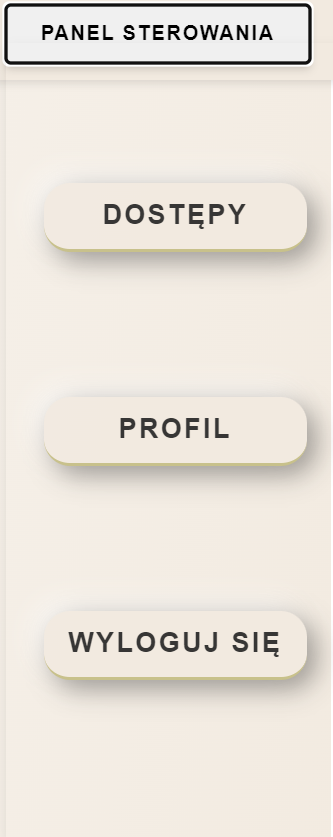
\includegraphics[scale=0.35]{photos/panel_sterowania_pracownika.png}
    \caption{Panel sterowania pracownika}
    \label{fig:login}
\end{figure}

\newpage

\noindent Po kliknięciu w opcje "Dostępy" zostanie wyświetlona lista dostępów do drzwi, które zostały przydzielone pracownikowi:
\begin{figure}[h]
    \centering
    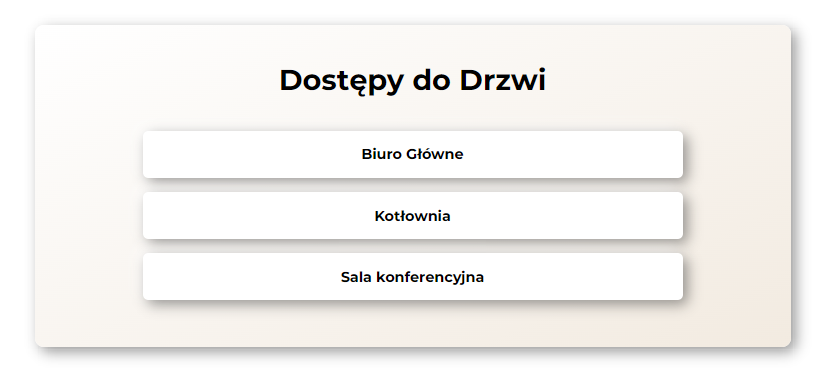
\includegraphics[scale=0.5]{photos/dostepy_do_drzwi_pracownika.png}
    \caption{Lista dostępów do drzwi pracownika}
    \label{fig:login}
\end{figure}

\subsection{Profil Administratora}
\noindent Administartor analogicznie jak pracownik po zalogowaniu zostanie przekierowany na stronę swojego profilu, 
natomiast panel sterowania będzie wyglądał następująco:
\begin{figure}[h]
    \centering
    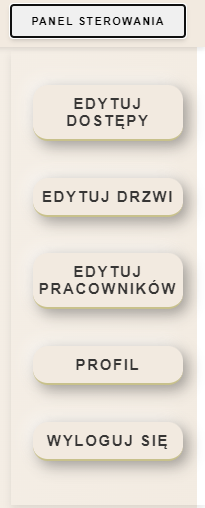
\includegraphics[scale=0.6]{photos/panel_sterowania_administratora.png}
    \caption{Panel sterowania administratora}
    \label{fig:login}
\end{figure}


\newpage

\subsubsection{Edyowanie dostępów}
\noindent Administrator po kliknięciu w opcje "Edytuj dostępy" zostanie przekierowany na stronę, gdzie będzie mógł edytować dostępy do drzwi.
Z listy wybieranej może wybrać pracownika, któremu chce zmienić dostęp do drzwi, a następnie z listy rozwijanej wybrać drzwi, które chce przydzielić pracownikowi.
Po kliknięciu w przycisk "Przydziel dostęp" zostanie zapisana zmiana w bazie danych. Poniżej 
znajduje się lista wszystkich dostępów do drzwi, które zostały przydzielone pracownikom. Administartor
może usunąć dostęp klikając w przycisk "Usuń".
\begin{figure}[h]
    \centering
    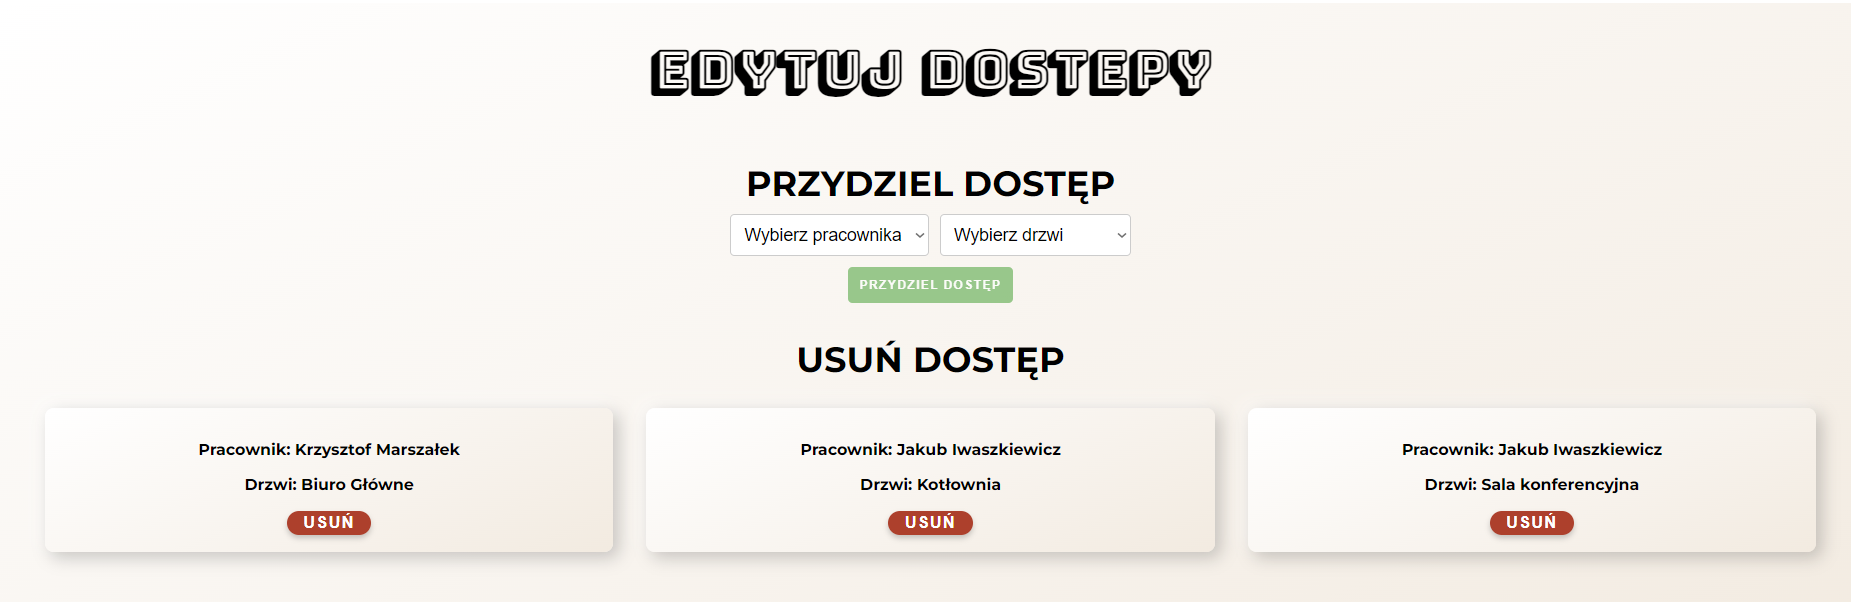
\includegraphics[scale=0.3]{photos/edytowanie_dostępów.png}
    \caption{Edytowanie dostępów}
    \label{fig:login}
\end{figure}


\subsubsection{Edytowanie drzwi}
\noindent Administrator po kliknięciu w opcje "Edytuj drzwi" zostanie przekierowany na stronę, 
gdzie będzie mógł edytować drzwi. Funkcjonalnośc dodawania drzwi wygląda w taki sposób, że administratorm
musi podać nazwę drzwi oraz jego opis. Po kliknięciu w przycisk "Dodaj" zostanie zapisana zmiana w bazie danych.
Poniżej znajduję się lista wszystkich drzwi z nazwami, które zostały dodane do systemu. Administrator może usunąć drzwi klikając w przycisk "Usuń".

\begin{figure}[h]
    \centering
    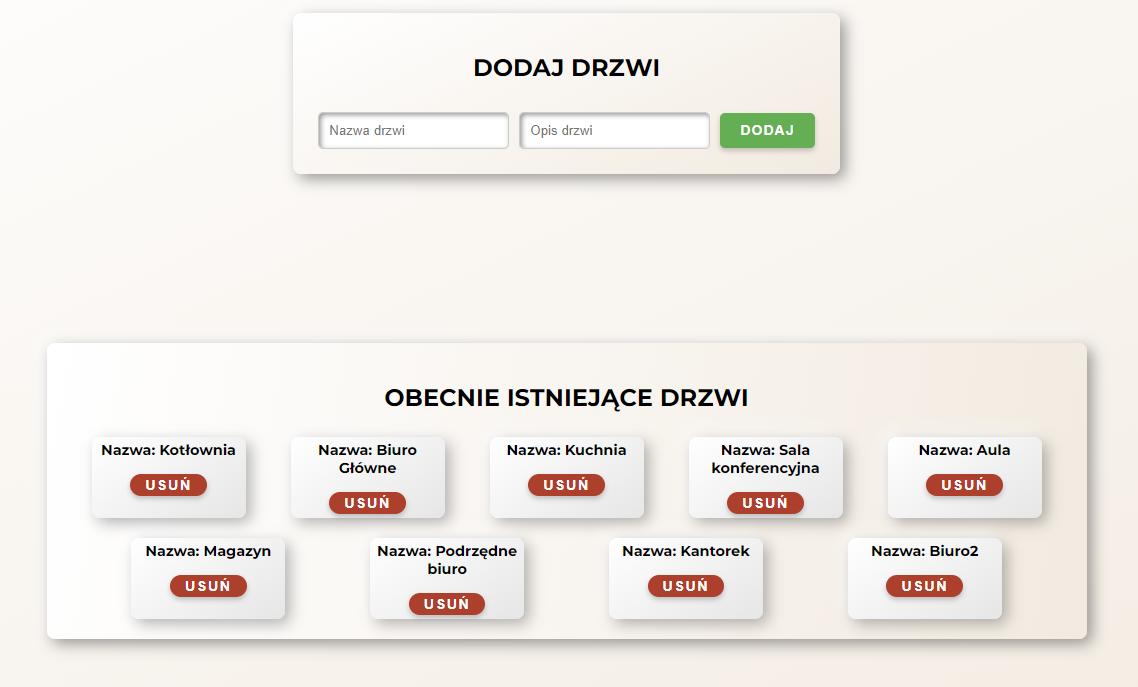
\includegraphics[scale=0.45]{photos/edytowanie_drzwi.png}
    \caption{Edytowanie drzwi}
    \label{fig:login}
\end{figure}

\subsubsection{Edytuj pracowników}
\noindent Administrator po kliknięciu w opcje "Edytuj pracowników" zostanie przekierowany na stronę,
gdzie będzie mógł edytować pracowników. Funkcjonalność dodawania pracownika
 wygląda w taki sposób, że administrator musi podać imię, nazwisko, email oraz hasło pracownika. 
 W każdej chwili może odsłonić hasło klikając przycisk "Pokaż hasło". Po kliknięciu 
 w przycisk "Dodaj pracownika" zostanie zapisana zmiana w bazie danych. Ponizej 
 znajduje się lista wszystkich pracowników, którzy zostali dodani do systemu.
  Administrator może usunąć pracownika klikając w przycisk "Usuń". W przypadku klinęcia usuń, wyskoczy 
  potwierdzenie usunięcia pracownika.
\begin{figure}[h]
    \centering
    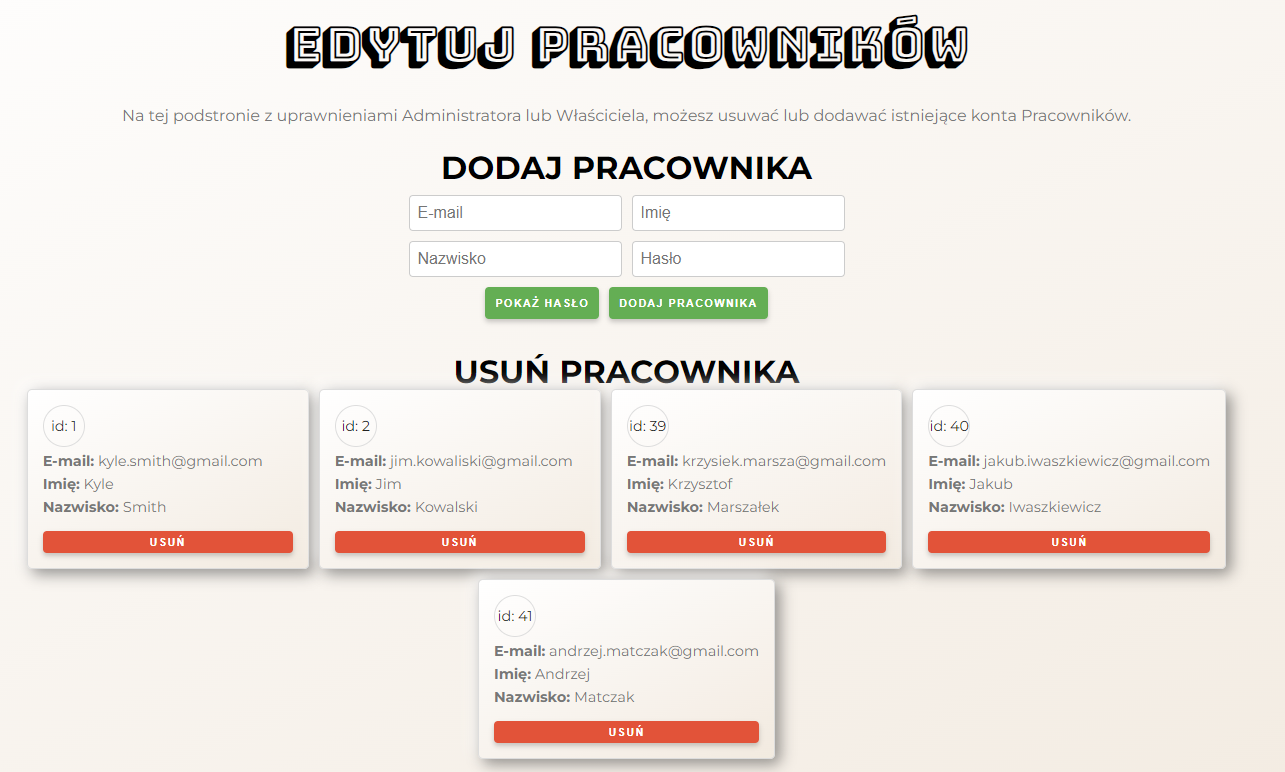
\includegraphics[scale=0.48]{photos/edytowanie_pracownikow.png}
    \caption{Edytowanie pracowników}
    \label{fig:login}

\end{figure}

\newpage

\subsection{Profil właściciela}
\noindent Właściciel analogicznie jak pracownik i administrator po zalogowaniu zostanie 
przekierowany na stronę swojego profilu. Właściciel ma dostęp do wszystkich opcji, które są dostępne 
dla administratora, oraz do dodatkowych opcji, takich jak "Dodaj przywileje" oraz "Usuń przywileje".

\begin{figure}[h]
    \centering
    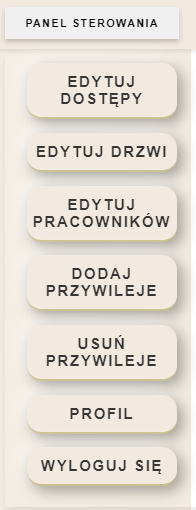
\includegraphics[scale=0.45]{photos/panel_sterowania_wlasciciela.png}
    \caption{Panel sterowania właściciela}
    \label{fig:login}
\end{figure}



\subsubsection{Edycja przywilejów}
\noindent Właściciel po kliknięciu w opcje "Edytuj przywileje" zostanie przekierowany na stronę,
na której może przyznać przywileje administratora wybranemu pracownikowi. Na tej podstronie zostaną 
wyświetleni wszyscy pracownicy. Właściciel może wybrać pracownika, któremu chce przyznać przywileje 
administratora. Po kliknięciu w przycisk "Dodaj jako Admina" zostanie zapisana zmiana w bazie danych.
W momecnie kiedy pracownik zostanie dodany jako administrator, mogą mu zostać przyznane przywileje właściciela.
\begin{figure}[h]
    \centering
    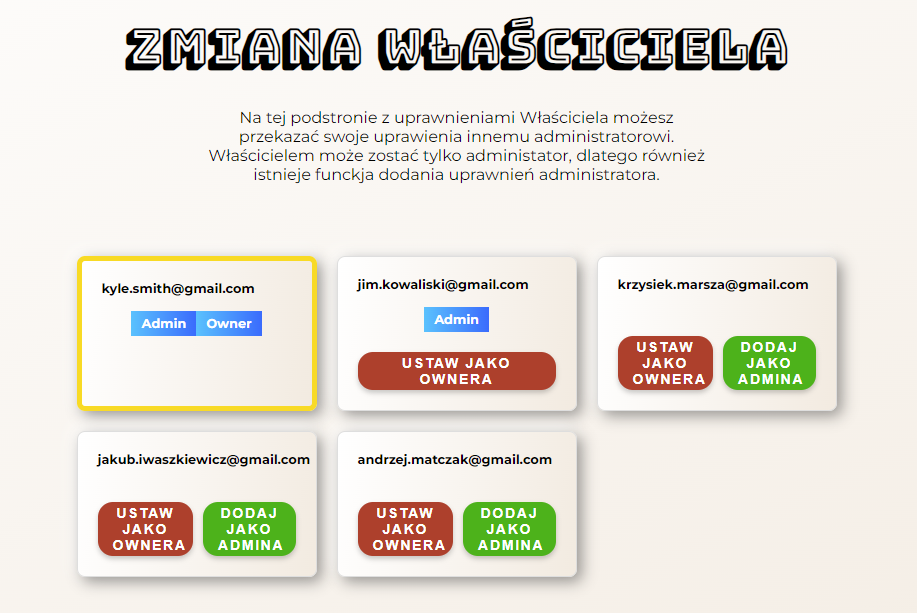
\includegraphics[scale=0.45]{photos/edytowanie_przywilejow.png}
    \caption{Edytowanie przywilejów}
    \label{fig:login}
\end{figure}
\newpage

\noindent W momencie kiedy właściciel przyzna przywileje administratora wybranemu pracownikowi, 
zostanie wyświetlony popout, który pyta właściciela czy chce przyznać przywileje właściciela wybranemu pracownikowi. Po 
kliknięciu w przycisk "Tak" zostanie zapisana zmiana w bazie danych.

\begin{figure}[h]
    \centering
    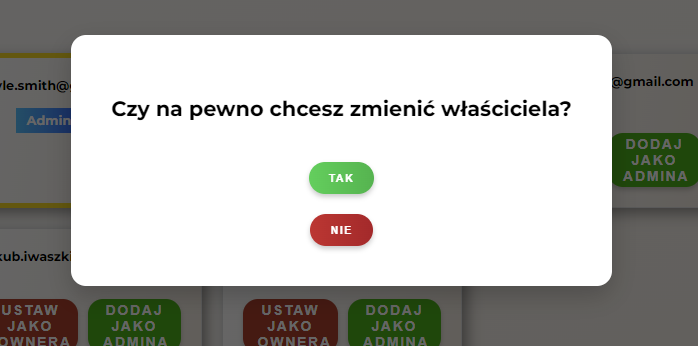
\includegraphics[scale=0.45]{photos/potwierdzenie.png}
    \caption{Potwierdzenie zmiany właściciela}
    \label{fig:login}
\end{figure}

\subsubsection{Usuwanie przywilejów}
\noindent Właściciel po kliknięciu w opcje "Usuń przywileje" zostanie przekierowany na stronę,
na której może usunąć przywileje administratora wybranemu pracownikowi. Na tej podstronie zostaną
wyświetleni wszyscy pracownicy z uprawieniami administratora. Właściciel może wybrać pracownika, któremu chce usunąć przywileje klikając
przycisk "Odbierz uprawnienia". Po kliknięciu w przycisk "Usuń jako Admina" zostanie zapisana zmiana w bazie danych:
\begin{figure}[h]
    \centering
    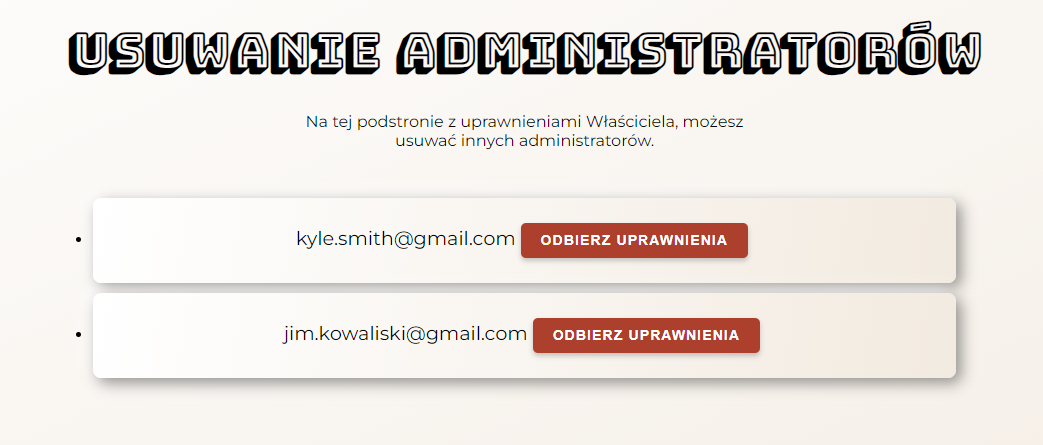
\includegraphics[scale=0.45]{photos/usuwanie_przywilejow.png}
    \caption{Usuwanie przywilejów}
    \label{fig:login}
\end{figure}
\newpage
\section{Podsumowanie}

\subsection{Wnioski}

Tworzenie aplikacji internetowej czy aplikacji mobilnej to 
bardzo złożona procedura wymagająca od progamisty bardzo złożonej 
wiedzy na temat narzędzi jak i samego wykorzystania narzędzia. 
Naszym ułatwieniem było to że jedna osoba z grupy już wcześniej 
przez jakiś czas miała do czynienia z narzędziem React.js co 
pozwoliło nam na w miare swobodne nauczenie się Express.js'a 
który pozwolił nam na ułożenie sobie wszystkiego w głowie a 
potem przelanie wszystkiego na kod. 
Pierwszą rzeczą jaką musieliśmy zrobić to wygląd graficzny 
naszej aplikacji która została wykonana w Figmie - 
samo znalezienie odpowiedniego narzędzia do tego i 
nauczenie się go było trudnym zadaniem, a 
co dopiero znalezienie palety kolorów, 
czcionek czy stylu naszej aplikacji - 
która i tak w trakcie programownia 
została nieco zaniechana przez brak czasu. 
Kolejnym wyzwaniem było rozpisanie funkcjonalności
jak i zostosowanie się do nich i wykorzystanie ich w Expressjs'ie.
Następnym wyzwaniem było połączenie się z bazą danych za pomocą Prisma,
co znacznie ułatwiło nam pracę z backednem.
W naszym projekcie React.js odegrał fundamentalną rolę, stanowiąc kręgosłup interfejsu użytkownika. Wykorzystanie tej biblioteki umożliwiło nam stworzenie dynamicznych, interaktywnych i responsywnych widoków, które dopasowują się do różnorodnych potrzeb użytkowników. Dzięki modularnej naturze React, nasz zespół był w stanie efektywnie zarządzać kodem, tworząc reużywalne komponenty, które znacząco przyspieszyły rozwój aplikacji.

Kluczowym elementem naszej pracy z React.js było zastosowanie zaawansowanych funkcji zarządzania stanem i cyklu życia komponentów. Hooki takie jak useState i useEffect odegrały zasadniczą rolę w dynamicznym zarządzaniu danymi aplikacji, umożliwiając natychmiastową reakcję interfejsu na zmiany.

Następnym krokiem było stworzenie podstron dla każdego rodzaju użytkownika 
oraz zaimpelementowanie React Router Dom, który pozwolił nam na
przekierowanie użytkownika na odpowiednią podstronę w zależności od jego uprawnień.
Kolejnym krokiem było stworzenie interfejsu graficznego dla każdej podstrony.
Wykorzystaliśmy do tego bibliotekę SASS, która pozwoliła nam na
zastosowanie styli w naszej aplikacji. 


\subsection{Możliwości rozwoju}

Dzięki zastosowaniu express.js'a jako tak na prawdę osobnej aplikacji, skalowalność aplikacji jest bardzo prosta, od strony serwerowej na pewno zabrakło możliwości napisania o odzyskanie zgubionej karty, jak i możliwości otworzenia drzwi w sposób zdalny (na stronie a nie przy pomocy karty) przez pracownika. Kolejną rzeczą jaką bym dołożył, to zwiększona ilość przechowywanych informacji przez naszą bazę danych pod względem wykonywanych działań przez pracowników (zapisywanie w bazie danych informacji o tym że ktoś przeszedł o tej godzinie przez te drzwi) jak i informacji na temat wykonywanych działań przez administratorów (zapisywanie informacji o tym że ktoś dodał pracownika lub właściciel został zmieniony również widoczny dla wszystki administratorów).

Jeżeli chodzi o interfejs graficzny to przez brak czasu niektóre elementy nie zostały w 100\% wystylizowane i niektóre mogą wyglądać nieco inaczej niż wszystkie - właśnie przez nie wykorzystanie pełnego potencjału komponentów reactowych i oddelegowywanie ich i wykorzystywanie we wszystkich podstronach, gdzie czasem mamy komponent w tym samym pliku co element wykorzystujący komponent, zamiast ulokowanego w innym pliku, gdzie jest to standardowa procedura dla Reacta.

Sama aplikacja może zostać rozwinięta przez jeszcze bardziej zaawansowane elementy, takie jak odzyskiwanie hasła, dwuetapowa weryfikacja, wysyłanie wiadomości do współpracowników, lecz zabrakło nam niestety czasu. Jeżeli pozwoli nam motywacja to prawdopodobnie będziemy chcieli ją dostosować do standardów rekrutacyjnych i będzie naszą pomocą w znalezieniu praktyk na wakacje.
\newpage
\listoffigures
\listoftables
\end{document}

